\section{Algebraic Multigrid} \label{sec_amg}
\subsection{Introduction}
As mentioned earlier, the most common way to solve a SPD system is to use
conjugate gradient preconditioned with SSOR (PCG-SSOR). In this research, we
will compare the calculation time using PCG-SGS, which is PCG-SSOR with a
damping factor equals to unity, with the time needed by CG 
preconditioned with an algebraic multigrid method. This is not a new idea: the 
first multigrid methods developed were geometric multigrid used as stand-alone 
solvers. In many applications, they achieve the so-called ``textbook multigrid
efficiency'', i.e. ``the solution to the governing system of equations [is
attained] in a computational work that is a small multiple of the operation
counts associated with discretizing the system'' \cite{textbook_eff}. However, 
in many other applications, multigrid methods, and particularly algebraic 
multigrid methods, cannot achieve such efficiency \cite{k_cycle}. In
such cases, they are often used as preconditioner for Krylov subspace methods. 
AMG make  very good preconditioners because they reduce all the error modes. Of
course, some modes may not be accelerated which can significantly degrades the 
efficiency of AMG as preconditioner. In \cite{amg_pn}, the authors used an 
algebraic multigrid method to precondition the Krylov solver for the even-parity 
finite element-spherical harmonics (FE-$P_N$) method. The AMG preconditioner 
resulted in a 60\% reduction in the solution time compared to ILU(0) 
preconditioning and even more reduction compared to SSOR preconditioning. 

We will employ and compare two multigrid approaches: one from the ML package
\cite{ml_guide} from the Trilinos library and the AGMG code \cite{agmg_guide}. 
ML is a multigrid preconditioning package that uses a smoothed aggregation 
algebraic multigrid to build a preconditioner for a Krylov method. AGMG is an 
aggregation-based algebraic multigrid code (written in Fortran 90).

We describe the multigrid principles, using first a two-grid setting. Consider
the following system:
\begin{equation}
  \bs{A}_f u_f = b_f
\end{equation}
defined on the fine grid $\mathbb{T}_f$.  The two-grid algorithm is given by :
\begin{enumerate}
  \item Perform $\nu_1$ pre-smoothing iterations using a smoother (e.g., Jacobi,
    Gauss-Seidel or ILU) using an initial guess $u_0$: $u = S^{\nu_1}(u_0,b_f)$
  \item Compute the residual on the fine grid $\mathbb{T}_f$ and restrict it to
    the coarse grid $\mathbb{T}_c$: $r_c = \bs{R}(b_f-\bs{A}_f u)$
  \item Solve with a direct solver the system on the coarse grid: 
    $v=\bs{A}_c^{-1} r_c$
  \item Interpolate the coarse grid correction to the fine grid and add the
    correction to $u$: $u \leftarrow u+\bs{P}v$
  \item Perform $\nu_2$ post-smoothing iterations: $u = S^{\nu_2}(u,b_f)$
\end{enumerate}
When using AMG, the matrix $\bs{A}_c$ on the coarse grid is given by the Galerkin
approximation:
\begin{equation}
  \bs{A}_c = \bs{R}\bs{A}_f \bs{P},
\end{equation}
where $\bs{P}$ is a prolongation matrix and $\bs{R}$ is a restriction matrix.
Solving the system $\bs{A}_c v = r_c$ on the coarse grid is generally very
expansive, therefore this step is recursively replaced by $\gamma$
applications of the  two-grid
methods until the system can be efficiently inverted with a direct solver.
This yields the multigrid method. When $\gamma = 1$, respectively $\gamma =
2$, the multigrid method is said to use a $V-$cycle, respectively a $W-$cycle:
\begin{figure}[H]
  \centering
  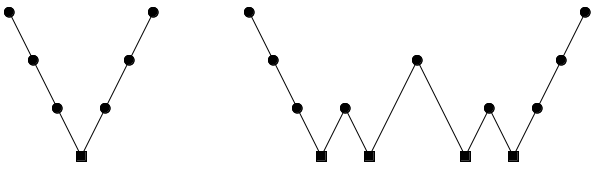
\includegraphics[width=0.5\textwidth]{./Dsa/v_w_cycles}
  \caption{$V-$ and $W-$cycles}
\end{figure}
A dot represents a smoothing operation and a square a direct inversion. The grid 
transfer operators are symbolized by lines.

For the coarsening step, both geometric and algebraic multigrid methods are 
based on the concept of smooth error. The difference between the two methods 
is that for geometric multigrid method, after the smoothing step, the error 
is \emph{geometrically} smooth relative to the coarse grid \cite{review_amg}. 
For algebraic multigrid methods, there might not be any grid and thus, only 
the properties of the matrix can be used. Therefore, the geometrical smoothness 
of the error cannot be used anymore. In fact, after the smoothing step, the 
error may be not smooth at all from the geometrical point of view. The reason 
is that the error is considered smooth when the smoother does not change the 
solution significantly anymore \cite{amg_course}:
\begin{equation}
  \|Se\|_{\mc{H}} \approx \|e\|_{\mc{H}}
\end{equation}
where $S$ is the smoother, $e$ is the error, and $\|u\|_{\mc{H}} =
\sqrt{(u,u)_{\mc{H}}}$ is the norm associated to the scalar product:
\begin{equation}
  (u,v)_{\mc{H}} = \(\bs{A}u,v\)_2.
\end{equation}
Among the algebraic multigrid methods, there are three main different 
types: the classical Ruge-Stueben AMG (also known as interpolation method), 
the plain aggregation AMG, and the smoothed aggregation AMG. ML uses 
smoothed aggregation AMG and AGMG uses plain aggregation AMG. The difference 
between theses methods is the coarsening step. The coarsening step is the 
most important step because if the coarsening is too fast, the convergence 
rates will decrease. However, if the coarsening is too slow, a lot of memory 
may be required to solve the problem. For classical Ruge-Stueben methods, 
each variable of the coarse grid is also a variable in the fine grid whereas 
for the aggregation methods, the variables of the fine grid are aggregates in
variables of the coarse grid. There is no simple identification between the 
variables of the fine grid and the coarse grid. However, all the algebraic
multigrid methods uses the  very important concept of strongly dependent
variables \cite{amg}:
{\definition{Given a threshold value of $0 \leq \theta \leq 1$, the variable
  $u_i$ strongly depends on the variable $u_j$ if:
  \begin{equation}
    -a_{ij} \geq \theta \max_{k \neq i} \(-a_{ik}\)
  \end{equation}}}
$a_{ij}$ must be of the same order of magnitude than the largest
off-diagonal in equation $i$ or $j$. A related definition is:
{\definition{If the variable $u_i$ strongly depends on the variable $u_j$,
then the variable $u_j$ strongly influences the variable $u_i$.}}\\
The idea behind the strong dependence is that if the coefficient $a_{ij}$ is
large, then a small change in the $j^{th}$ variable will have an important
effect on the $i^{th}$ variable. Thus, it is probably a good idea to use the
$j^{th}$ variable to interpolate the $i^{th}$ variable or to couple these two
variables in an aggregate. This can be easily seen using the concept of
smoothed error. For the error to be considered to be smoothed, assuming that
$\bs{A}$ is a $M$-matrix, i.e., off-diagonal entries of the matrix are less 
than or equal to zero and the real parts of the eigenvalues of the matrix 
are positive, the following relationship needs to be satisfied for most $i$ 
\cite{amg}:
\begin{equation}
  \sum_{j\neq i} \(\frac{|a_{ij}|}{a_{ii}}\) \(\frac{e_i-e_j}{e_i}\)^2 \ll 1
  \label{ineq}
\end{equation}
where $e_i$ is the error associated to the variable $i$. Since the left side 
of \cref{ineq} is positive, all the products must be small which means that 
at least one of the two terms of each product has to be small. When the
$i^{th}$ variable strongly depends on the $j^{th}$ variable 
$\frac{|a_{ij}|}{a_{ii}} \approx 1$, $e_i-e_j$ must be small
or equivalently $e_i \approx e_j$. This means that the error varies slowly
in the direction of strong connection. That is the reason why the coarsening
is done along these directions.

\subsection{Classical AMG (interpolation method)}
For classical AMG, the variables of the coarse grid are a subset of the
variables of the fine grid. The variables can be split in two disjoint
sets: $C$ that contains all the coarse variables and $F$ that contains all the
other variables. Thus, the error on the fine grid is given by \cite{review_amg}:
\begin{equation}
  e_{c,i} = (\bs{P} e_f)_i = \left\{
  \begin{aligned}
    & e_{c,i} & \textrm{ if } i\in C\\
    & \sum_{k\in B_i} w_{ik} e_{c,k} & \textrm{ if } i\in F
  \end{aligned}
  \right.
\end{equation}
where $B_i$ is a subset of $C$ whose variables are called interpolatory
variables. $B_i$ should be a small subset of $C$ to keep $\bs{A}_c$ sparse.
Now, we assume that $\bs{A}$ is a $M$-matrix and we review two typical 
interpolation methods:
\begin{description}
  \item[Direct interpolation:] First, we define the neighborhood of the
    $i^{th}$ as the set $N_i = \{ j \in C \cup F: j\neq i, a_{ij} \neq 0\}$.
    After the smoothing step, we can write locally:
    \begin{equation}
      e_i \approx -\frac{\(\sum_{j\in N_i} a_{ij} e_j\)}{a_{ii}}.
      \label{e_locally}
    \end{equation}
    If $B_i$ contains the variables which are strongly dependent on the
    $i^{th}$ variables, we have:
    \begin{equation}
      \frac{1}{\sum_{k\in B_i} a_{ik}} \sum_{k \in B_i} a_{ik} e_k \approx 
      \frac{1}{\sum_{j\in N_i} a_{ij}} \sum_{j \in N_i} a_{ij} e_j.
    \end{equation}
    Using this relation and \cref{e_locally}, we get the following formula for
    the weights of the interpolation:
    \begin{equation}
      w_{ik} = -\alpha_i \frac{a_{ik}}{a_{ii}}
    \end{equation}
    where $\alpha_i = \frac{\sum_{j\in N_i} a_{ij}}{\sum_{l \in B_i} a_{il}}$.
    Therefore, it is important that when the coarse variables are chosen,  
    that every variable in $F$ has enough strongly coupled
    variables in $C$ that are part of of $B_i$. If some of the off-diagonal
    entries are positive, the same development can be done as long as these
    positive terms are small, i.e., variables are not strongly coupled because
    of these terms. If the positive entries are large, the algebraically
    smooth error can oscillate. This can happen, for elliptic PDE, when 
    high-order finite elements are used or with bilinear elements on 
    quadrilateral meshes with large aspect ratios. This will negatively affect
    the performance of AMG.
  \item[More complex interpolations:] More complex interpolation schemes can
    be created but they reduce the sparsity of $\bs{P}$ and $\bs{R}$, increasing the
    size of $\bs{A}_c$. Moreover, the weakly-dependent variables will be 
    associated to smaller weights which makes them having a small effect. It
    can therefore be interesting to ignore the smallest values in the
    interpolation matrix and to rescale the others weights so that the sum of
    the weights does not change. This can slow down the convergence of the
    method but it will not make it diverge \cite{review_amg}.
\end{description}
A good rule, when coarsening the grid, is to try to have the set of coarse 
variables to form a maximally independent set, i.e. a maximal set where the 
coarse variables are not strongly coupled to each others, and the variables 
in $F$ are surrounded by the variables in $C$. We call $B_i^S$ the set of all 
strongly connected neighbors of $u_i$:
\begin{equation}
  B_i^s = \{ v_j \in B_i | -a_{ij} \geq \theta \max_{k\neq i}(-a_{i,k})\}.
\end{equation}
The interpolatory nodes $C_i$ are:
\begin{equation}
  C_i = B_i^s \cap C.
\end{equation}
Adding variables in $C_i$ increases the quality of the interpolation but
it diminishes the sparsity of the interpolation matrix and increases the
size of $\bs{A}_c$ which increases the computational cost of the method.
Thus, we want that for every variable $u_i$ in $F$, every $u_j \in B_i^s$
should be in $C_i$ or strongly connected to at least one variable in
$C_i$. This rule will make sure that the interpolation is of a good enough
quality. We also want $C$ to be a maximal subset of the variables such that 
the variables in $C$ are not strongly connected to each others. This ensures 
that the coarsening is fast enough.

\subsection{Smoothed aggregation: the ML package}
In a similar way than for the classical AMG, the smoothed aggregation
method uses the concept of strong connections. The theory for plain
aggregation method showed that the convergence bound depends of the number
of levels \cite{amg_unstruc}. This is a major flaw of the plain aggregation
method which was also observed in practice. To counter this, the smoothed
aggregation was created. This method converges fast for a lot of different 
problems including the ones with anisotropic and discontinuous coefficients.
  
When using a smoothed aggregation scheme, the smoothed interpolation operators,
$\bs{P}_k$, are the transpose of the coarsening operators,
$\bs{R}_k=\bs{P}_k^T$. Therefore, when the $\bs{P}_k$ are built, the
coarsening is known. First, the graph of the matrix is constructed: if the element
$(i,j)$ or $(j,i)$ of the matrix is non-zero, an edge is built between the
vertex $i$ and the vertex $j$ \cite{ml_guide}. Second, the vertices are
aggregated. When using ML on a single processor, two aggregation schemes can
be used: the uncoupled scheme or the maximally independent sets (MIS) scheme. 
The uncoupled scheme attempts at building aggregates of size $3^d$ where $d$ is the
dimension of the problem. The algorithm works as follows \cite{mis}:
\begin{description}
  \item[Step 1:] As long as there are points not adjacent to an aggregate:
    \begin{enumerate}
      \item Choose a point which is not adjacent to an aggregate. This point
        is a new root point.
      \item Define a new aggregate as the root point and its neighbors.
    \end{enumerate}
  \item[Step 2:] Add all the points left to the existing aggregates or form a
    new aggregates with them.
\end{description}
The MIS scheme used in ML applied the MIS algorithm of \cite{graph_coloring} to
the graph produced by the matrix $\bs{A}^2$. These two coarsening 
schemes use a fixed ratio of coarsening between levels. Once the aggregation is 
done, a tentative prolongator matrix, $\bs{\tilde{P}}_k$ is constructed 
\cite{mis}. A example of $\bs{\tilde{P}}_k$ is given by:
\begin{equation}
  \bs{\tilde{P}}_k(i,j) = \left\{
  \begin{aligned}
    &1 &\textrm{if }i^{th}\textrm{ point is contained in }j^{th}\textrm{
    aggregate}\\
    & 0 &\textrm{otherwise}
  \end{aligned}
  \right.
\end{equation}
This tentative prolongator could be used as prolongator but smoothing it
allows to have a more robust scheme. Let $\bs{S}_k$ be a smoother, for example
damped Jacobi, then the prolongator matrix is given by:
\begin{equation}
  \bs{P}_k = \bs{S}_k \bs{\tilde{P}}_k.
\end{equation}

Like for classical AMG, it can be interesting to ignore small values in
the graph since the smoother will be ineffective for the weakly coupled
variables. In ML, there is a drop tolerance, $tol$, that is used to ignore
entries in the graph if $|a_{ij}| \leq tol\ \sqrt{|a_{ij} a_{jj}|}$. The
tolerance, whose default value is zero, can be changed.  In ML, when the 
matrix is SPD, CG is used to determine the Jacobi damping parameter, which 
is an approximation of the spectral radius.

By default, the coarsening is stopped when the number of variables is less 
or equal than 128.

\subsection{Plain aggregation: the AGMG code}
Unlike ML, in AGMG the prolongator is not smoothed which results in a
cheaper setup and a decrease of required memory \cite{agmg2}. However, 
the scheme could be less robust. To counteract this weakness, 
the aggregation scheme is more complicated. Coarsening algorithms that control
the size of the aggregates tends to produce a few badly shaped aggregates.
Since the convergence of AMG is bounded by the worst aggregate, even a small 
number of badly shaped aggregates can have a huge impact on the convergence. 
In AGMG, the aggregation algorithm has as input the upper bound of the 
two-grid condition number $\bar{\kappa}_{TG}$. When the aggregates are constructed,
their quality is checked. Obviously, this increases the cost of the coarsening
and it is important that the coarsening is fast enough. Since the algorithm 
does not control the size of the aggregates, it is difficult to control the 
speed of the coarsening. However, controlling the condition number is much 
more interesting than controlling the coarsening speed. If the algorithm 
controls the condition number, it will not create bad aggregates but instead, it 
may create a few aggregates with a size below the target size but this 
does not affect the efficiency of the method in a noticeable way \cite{agmg2}. 

In AGMG, the aggregation is done by a few passes of a pairwise aggregation 
algorithm. This allows the computation of the aggregate quality to remain very 
simple and to keep the cost per iteration low. The advantage of controlling the 
condition number becomes even more important when a $K-$cycle or Krylov-cycle is 
used instead of the more common $V-$ or $W-$cycles. The difference between the 
$K-$cycle and the $V-$ or $W-$cycle is that the $K-$cycle uses recursively a 
few iterations of a Krylov solver preconditioned by a coarser grid to solve 
the coarse grid problem in the two-grid algorithm \cite{k_cycle}. This scheme 
is nonlinear and requires, when the system is SPD, to use flexible CG 
\cite{fcg_2,fcg_3,fcg_4,fcg} as Krylov solver. The advantage of the $K-$cycle is 
an increased robustness compared to $V-$ and $W-$cycle. Even when the condition 
number of the two-grid method is large, the convergence properties of the 
$K-$cycle can be independent of the number of levels \cite{k_cycle}. The 
computational cost of $K-$cycle is about the same than the cost of the 
$W-$cycle. If the number of unknowns does not decrease sufficiently from one 
level to the next, the $K-$cycle at one level is replaced by a $V-$cycle at 
this same level. The idea of $K-$cycle is not new since it was already used 
in Algebraic MultiLevel Iteration (AMLI) methods \cite{amli}. AMLI are 
hierarchical basis methods stabilized by the recursive calls of preconditioner 
created thanks to a coarse level. 

Next, we explain the coarsening step in AGMG for $M-$matrix (SPD). 
We want to create nonempty disjoint sets $G_k$, $k=1,\hdots,n_c$ called 
aggregates with each one of them associated to a variable in a coarser grid. 
Some of the unknowns are not associated to any variables in the coarse grid 
and they are in the set $G_0$. The prolongation matrix is given by:
\begin{equation}
  \bs{P}_{ij} = \left\{
    \begin{aligned}
      1& \textrm{ if }i\in G_j\\
      0& \textrm{ otherwise}
    \end{aligned}
    \right.
\end{equation}
Thus, $\bs{P}$ has at most one non-zeros entry by row. A row is only
composed of zeros if the variable associated to this row is in $G_0$. A
simple method to form the high quality aggregates of a given size would be
to test all the possibility. For an obvious reason, this cannot be done in
practise. Instead, in AGMG several passes of pairwise aggregation are done. 
The reason is that when two variables are aggregated, the quality factor of 
the aggregate $\kappa(G)$ is given by: 
\begin{equation}
  \kappa(\{i,j\}) = \frac{-a_{ij} +\(\frac{1}{a_{ii}+s_i+2a_{ij}}+
  \frac{1}{a_{jj}+s_j+2 a_{ij}}\)^{-1}}{-a_{ij}+\(\frac{1}{a_{ii}-s_i}+
  \frac{1}{a_{jj}-s_j}\)^{-1}}
\end{equation}
where $s_i = - \sum_{j\neq i} a_{ij}$. $\kappa$ is only given by the
off-diagonal entry connecting these two unknowns, their respective diagonal
entries, and the sum of all off-diagonal elements in the corresponding rows.
As $|G|$ increases, it becomes more and more costly to compute
$\kappa(|G|)$. However, checking that $\kappa(|G|)$ is below a given
threshold $\bar{\kappa}_{TG}$ is relatively cheap. It is sufficient to
check that:
\begin{equation}
  \bar{\kappa}_{TG} \bs{A}_G - \bs{M}_G\(\bs{I}-\bs{1}_G \(\bs{1}_G^T
  \bs{M}_G\bs{1}_G\)^{-1}\bs{1}_G^T\bs{M}_G\)
\end{equation}
is nonnegative definite. This can be done in $\mc{O}(|G|^3)$ operation
by verifying that the Cholesky factorization exists, i.e., there is no negative
pivot. Therefore, $\kappa(|G|)$ does not need to be computed explicitly to
make sure that $\kappa(|G|) \leq \bar{\kappa}_{TG}$. The first pairwise
coarsening step is given by:
\begin{enumerate}
  \item Create the set $G_0$, i.e., create the set of variables which will
    not be aggregated.
  \item Choose an unknown and find among its unassigned neighbors the one
    that gives the smallest $\kappa(\{i,j\})$.
  \item Check that $\kappa(\{i,j\}) \leq \bar{\kappa}_{TG}$. If the
    condition is not verified, the variable is left unassociated in the coarse
    grid.
\end{enumerate}
To increase the size of the aggregates, the temporary coarse grid matrix
$\bs{\tilde{A}}_c$ is computed and the same process that the one we just
described is applied. The set $G_0$ cannot be changed and the quality factor
$\tilde{\kappa}(\{i,j\})$ needs to be adapted to reflect the quality of the
corresponding aggregate $\kappa(G_i\cup G_j)$ in the original matrix.
Therefore, the definition of $s_j$ is slightly modified:
\begin{equation}
  \tilde{s}_i = - \sum_{k \in G_i} \sum_{j \in G_i} a_{kj}.
\end{equation}
This change is there to ensure that $\tilde{\kappa}(\{i,j\})$ is a lower
bound of $\kappa(G_i \cup G_j)$. Thus, if $\tilde{\kappa}(\{i,j\}) \geq
\bar{\kappa}_{TG}$, the pair has to be rejected because it is impossible for
$\kappa(G_i \cup G_j)$ to satisfy the condition. An unique characteristic 
of this coarsening method is that you can, in theory, have an 
arbitrary number of pairwise coarsening passes without degrading the upper
bound of the condition number. In practise, however, the coarsening is
stopped if either a given number of passes has been done or the coarsening
factor has reached a target value. To conclude the explanation of the
coarsening step, we explain how unknowns are picked and how to pick between 
a pair $\{i,j\}$ and another $\{i,k\}$ if they have the same quality factor. 
If there is no priority rules, the coarsening would depend of the ordering 
of the variables or the way off-diagonal entries are stored. In AGMG, the 
rule chosen tries to increase the regularity of the aggregates because in 
practise, this increases the coarsening speed of the coarser levels. Even 
if the coarsening step tries to create regular aggregates on regular grids, 
the results are still quite good for unstructured grids \cite{agmg2}. The 
priority rule consists of using a Cuthill-McKee permutation 
\cite{cmk} to renumber the variables and to use the number associated to the 
variable as a priority number (the lower number has the priority). The 
Cuthill-McKee permutation works as follows: the number 1 is given to a node 
with minimal degree; the next numbers are given to its neighbors ordered by
increasing degree; then their neighbors are given a number by
increasing degree; the process is over when all nodes are numbered. There is
still some uncertainties in the numbering if there are several variables
with minimal degree or when several neighbors of a variables have the same
degree. However, these choices do not affect the
performance \cite{agmg2}. 

AGMG stops the coarsening when the number of variables is less or equal to
400.
